\documentclass[12pt,a4paper]{report}
\oddsidemargin=-5.00mm
\textwidth=170.00mm
\topmargin=-10.00mm
\textheight=240.00mm

\usepackage[pdftex]{graphicx}
%\usepackage{refcheck}
\usepackage{natbib}%\usepackage{harvard}
\usepackage{amsmath,amssymb}
\usepackage[blocks]{authblk}
\usepackage{indentfirst}
\usepackage{float}
\usepackage[linktoc=all]{hyperref}
\usepackage{color}
\usepackage{titlesec}
\usepackage{listings}
\lstset{frame=lrbt,xleftmargin=\fboxsep,xrightmargin=-\fboxsep}


%\input{../../../Notes/Preamble.tex}
%\input{latex_path/preamble.tex}
%\input{preamble.tex}

% - particular to this problem (vary easily)

\begin{document}
\title{WIM Description.}

%\author{L.G.~Bennetts\authorcr
%luke.bennetts@adelaide.edu.au}
%\affil{School of Mathematical Sciences\authorcr
%University of Adelaide\authorcr
%Adelaide 5005\authorcr
%Australia
%}

\author{T.D.~Williams\authorcr
timothy.williams@nersc.no}
\affil{Nansen Environmental and Remote Sensing Center\authorcr
Thorm{\o}hlensgate 47\authorcr
5006 Bergen\authorcr
Norway
}

\date{\today}
\maketitle

\tableofcontents
%\section{Introduction}
\chapter{Introduction}

%$\quad$\,\,\,\,
Text.

\chapter{Mathematical and physical background}

Text.


\section{Scattering model}
Text.

\subsection{Two-dimensional model: a single floe}

Text.
\cite{williams-etal2013-break2}
%%%%%%%%%%%%%%%%%%%%%%%%

%\begin{figure}[H]
%\begin{tabular}{cc}
%\includegraphics[scale=0.27]{xtra_figs/foto-conc79-setup.pdf}
%&
%\includegraphics[scale=0.27]{xtra_figs/foto-conc39-setup.pdf}
%\end{tabular}
%\caption{Set-up of the multiple floe experiments, with two different concentrations:  one at a higher concentration, about 79\% (left), and another at a lower concentration about 39\% (right).}
%\label{pic-mult-setup}
%\end{figure}

\chapter{Cron and Crontab} \label{cron}
%\input{CRON.tex}
In this chapter, after a brief introduction on \textit{Cron}, the user will learn how to check and modify a \textit{Crontab} file.
\section{Introduction}
\textit{Cron} is a software utility time-based for \textbf{Unix-like} operating systems. \textit{Crontab} is a text file that guides \textit{Cron} providing the time and nature of its operations; it is possible for every user to have a personal \textit{Crontab}. Every \textbf{minute} \textit{Cron} checks the uploaded \textit{Cronfile} comparing it to the \textbf{system} time. These tasks will run regardless of whether the user is actually logged into the system.
\section{Crontab editing}
The layout of the \textit{Crontab} file (fig. \ref{crnlay}) provides 5 inputs for time and 1 for the command:
\begin{figure}[h!]
\centering
\fbox{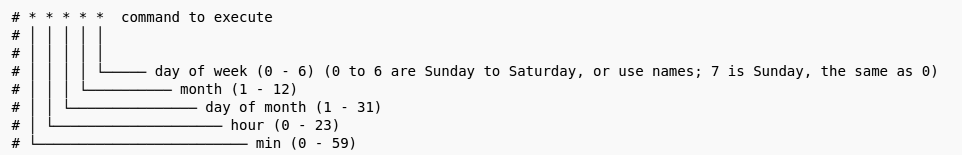
\includegraphics[width=1\textwidth]{crontablayout}}
\caption{\textit{Crontab} file's layout with explanation}
\label{crnlay}
\end{figure}
\begin{lstlisting}[language=bash]
# This is an example of a Crontab file
* * * * * /home/user/prog1.sh	# Every minute
15 * * * * /home/user/prog2.sh	# Every hour at min 15
# Comments don't interfere with the tab
12 18 * * * /home/user/prog3.sh	# Every day at 18:12
*/5 * * 1 * /home/user/prog4.sh	# Every 5 minutes of January
\end{lstlisting} 
\textbf{NOTE} - *\textbackslash \ will reiterate that command \\ \\
To modify the \textit{Crontab} a previously written file can be uploaded (\textit{i.e. mycrontab}) or it can be manually modified (this will change the current user's). \\
\begin{lstlisting}[language=bash]
$ crontab mycrontab 	# Uploading a personal Crontab
$ crontab -e	 	# Manually modifying the Crontab
\end{lstlisting}
\section{Crontab on Hexagon}
\textit{Cron} is working on \textbf{Hexagon} as well but since is a very busy and heavily stressed system there are a few precautions that should be remembered before setting up a \textit{Cron} job. \\ \\
First of all you should choose a \textit{node} in which set up your \textit{Crontab}. A \textit{node} is a connection, redistribution or communication point for a network. For more information please visit (\url{http://docs.hpc.uib.no/wiki/Main_Page}). \\
Another precaution is to use unique \textit{Crontab} file's names so that different set-ups will not be uploaded by mistake. \\ \\
Here is shown a complete procedure for a \textit{Crontab} setup in \textbf{Hexagon}: \\
\begin{lstlisting}[language=bash]
$ ssh hexagon		# Personal login on Hexagon

# Now a Cron-job is appended to a unique personal tab 
$ echo "* * * * * /home/user/prog.sh" >> prog_cron

$ ssh login1		# Login node1 (change number to change node)
$ crontab prog_cron	# Uploading unique Crontab
\end{lstlisting}
Now every minute \textit{Cron} will execute \textit{prog.sh} from \textit{node1}. \\ \\
\textbf{Remember} that the outputs of \textit{Cron} are shown in a virtual display hence are lost if not saved. It is possible to save the outputs by manually inserting a log, saving stdr.out or setting up an automatic e-mail service that will send to a specified address the outputs by adding the following line in the \textit{Crontab} file (\textbf{NB} before the jobs):
\begin{lstlisting}[language=bash]
$ MAILTO=user@domain.org
\end{lstlisting}



\chapter{Model's Inputs - last modification \today}

%%Model's Inputs Updating Procedure

In this chapter the user will be instructed on how to control the scripts used to download and storage the input files that will be used as initial conditions for the WIM model.\\
There are four products that are updated and/or stored daily:
\begin{itemize}
\item TOPAZ - Weekly Restart Files
\item WAMNSEA - Daily Waves 
\item ECMWFR - Daily Weather
\end{itemize}

\section{TOPAZ}
\subsection{Introduction}
\textbf{T}owards an \textbf{O}perational \textbf{P}rediction system for the North \textbf{A}tlantic European coastal \textbf{Z}ones, simply known as TOPAZ is a coupled ocean-sea ice data assimilation system for the North Atlantic Ocean and Arctic. It is the only operational, large-scale ocean data assimilation system that uses the ensemble Kalman filter. This means that TOPAZ features a time-evolving, state-dependent estimate of the state error covariance. \\ \\
In the regional Barents and Kara Sea forecast system (\textbf{BS1}), the TOPAZ (\textbf{TP4}) is used as an outer model in the nested system. Locally the TP4 model runs once a week for an 11 days period, with 9 days forecast, and produce initial and boundary conditions for the regional model BS1.
\subsection{Data Gathering}
The product consist of 3 different files:
\begin{itemize}
\item TP4restart\textit{YYYY\_ddd\_hh}\_mem001.a
\item TP4restart\textit{YYYY\_ddd\_hh}\_mem001.b
\item TP4restart\textit{YYYY\_ddd\_hh}ICE.uf
\end{itemize}
%ADD A BRIEF DESCRIPTION OF WHAT THE FILES ARE
These files are weekly uploaded to the main server of the forecast system, HEXAGON, the supercomputer service at the University of Bergen.
\begin{lstlisting}[language=bash]
$ ssh hexagon
\end{lstlisting}
%Model's Inputs Updating Procedure

In this chapter the user will be instructed on how to control the scripts used to download and storage the input files that will be used as initial conditions for the WIM model.\\
There are two products that are updated and/or stored from every week to every hour:
\begin{itemize}
\item TOPAZ - Weekly Restart Files
\item WAMNSEA - Daily Waves 
\end{itemize}

\section{TOPAZ}
\subsection{Introduction}
\textbf{T}owards an \textbf{O}perational \textbf{P}rediction system for the North \textbf{A}tlantic European coastal \textbf{Z}ones, simply known as TOPAZ is a coupled ocean-sea ice data assimilation system for the North Atlantic Ocean and Arctic. It is the only operational, large-scale ocean data assimilation system that uses the ensemble Kalman filter. This means that TOPAZ features a time-evolving, state-dependent estimate of the state error covariance.
\\ \\
In the regional Barents and Kara Sea forecast system (\textbf{BS1}), the TOPAZ (\textbf{TP4}) is used as an outer model in the nested system. Locally the TP4 model runs once a week for an 11 days period, with 9 days forecast, and produce initial and boundary conditions for the regional model BS1.
\subsection{Data Format}
The restart product consist of 3 different files that will provide initial conditions: \\
\begin{itemize}
\item \textbf{TP4restart\textit{YYYY\_ddd\_hh}\_mem001.a} - [\textbf{data}] initial conditions of the system.
\item \textbf{TP4restart\textit{YYYY\_ddd\_hh}\_mem001.b} - [\textbf{text}] information and instructions for the first file.
\item \textbf{TP4restart\textit{YYYY\_ddd\_hh}ICE.uf} - [\textbf{data}] informations about sea ice (localization, height, etc..).
\end{itemize}
Where \textbf{Y} is the Year, \textbf{d} is the day and \textbf{h} is the hour of the restarts release. \\ \\
\textbf{NB} - file names could change depending on the service.
\\ \\
These files are weekly uploaded to the main server of the forecast system Hexagon. They will be temporary stored in a working directory that is cleared every two weeks (or else depending on the needs of the server) hence the need of a script that will daily check and if needed archive and transfer the new data (see \ref{tparchv}).

\section{WAMNSEA}
%WE ARE USING WAM 10

\chapter{Scripts Protocol - \today}
For the daily forecast product, its storage and online delivery, the algorithm follows 3 main phases:
\begin{itemize}
\item \textbf{Inputs Download and Archiviation}
\item \textbf{Model Run}
\item \textbf{Post-processing and Storing}
\end{itemize}
\textbf{NB} All the scripts can be found on the \textit{GIT-HUB} directory (https://github.com/nansencenter/SWARP-routines). 
\\ \\
The following diagram shows the work directory:
\begin{figure}[h!]
\centering
\fbox{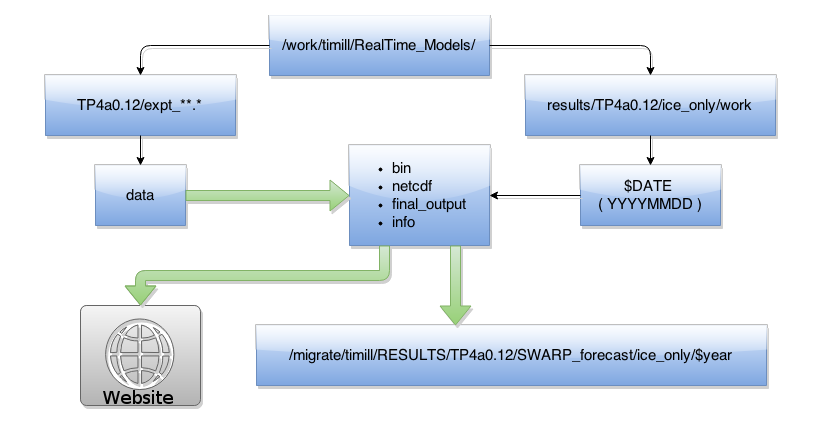
\includegraphics[width=1\textwidth]{work_dir}}
\caption{\textbf{**.*} indicates the experiment ran; \textbf{\$DATE} is the daily date (\textit{YYYYMMDD}) and the \textbf{green} arrows are operations done by the scripts described later in this chapter. }
\label{wrkdir}
\end{figure}
\\
\textbf{NB} It is possible that these directories will be changed and/or modified, please use caution and keep this log up to date if possible.

\section{Inputs Download and Archiviation}
\label{IDA}
The protocol consists in 2 scripts
\begin{itemize}
\item topaz\_archive\_restart.sh
\item wamnsea\_update.sh
\end{itemize}

\subsection{topaz\_archive\_restart.sh}
\label{tparchv}
\textbf{dir - forecast\_scripts}
\\ \\
The purpose of this script is to daily check the presence of new restarts for the Topaz model, collecting and store them. These are binary files produced by the \textit{Nansen Environmental and Remote Sensor Center} weekly and can be found on the super computer \textbf{Hexagon}.
\\ \\
The logic behind the script is to find all the files with \textbf{TP4restart} in their file-name and check their presence in a list of the stored files. If the file is on the list it has already been archived and the script will end otherwise will automatically add the new files to the list and to the archive (using a \textit{tar} compression protocol). Every operation will write a daily log that will be appended to a report delivered weekly to the forecast supervisor.
\\ \\
This script is regularly executed by \textbf{Cron} (see [\ref{cron}]) at 18:00 everyday.

\subsection{wamnsea\_update.sh}
\label{wamnseaupdate}
\textbf{dir - forecast\_scripts}
\\ \\
The goal of this script is to constantly update the wave analysis and forecast for the North and Barents sea. These are Netcdf files produced by \textit{met.no} and uploaded daily on \textbf{myocean}. 
\\ \\
The script will download every WAM product (both daily analysis and forecasts) present on \textbf{myocean} using a \textit{ncftp} protocol. If a product was already downloaded it will be substituted by the new one. The daily products are stored, a copy of them will be merged in a single file for every year.
\\ \\
This script is regularly executed by \textbf{Cron} (see [\ref{cron}]) every hour except for a time-out window (00:00/04:00) where it won't download any file because usually the files are uploaded after 03:00. If no new file is downloaded between 04:00 and 08:00 an email alert will be sent to the forecast supervisor.

\section{run\_forecast.sh}
\label{runforecast}
\textbf{dir - forecast\_scripts}
\\ \\
The script is a collection of 3 scripts:
\begin{itemize}
\item \textbf{topaz\_get\_restart.sh}
\item \textbf{make\_infile4forecast.sh}
\item \textbf{pbsjob.sh}
\end{itemize}
The last one will also launch the subscript \textbf{process\_FCresults.sh} described in \ref{processfcresults}.
\\ \\
The following diagram shows the script's main structure:
\begin{figure}[h!]
\centering
\fbox{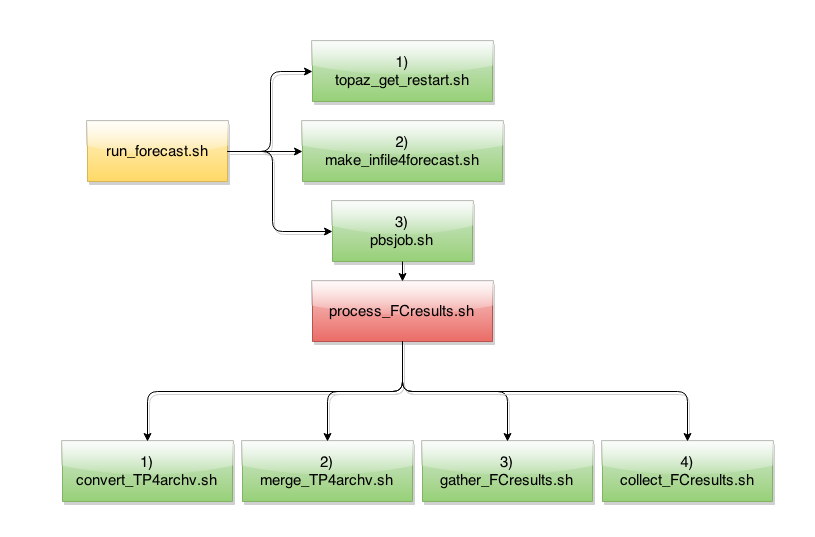
\includegraphics[width=1\textwidth]{run_FC}}
\caption{}
\label{runfc}
\end{figure}
\\ \\
First of all this scripts produces a text file named \textbf{datelist.txt} that contains all informations regarding the date of the run. It then launches the subscripts.
\\ \\
This script is regularly executed by \textbf{Cron} (see [\ref{cron}]) every day at 0200 - \textbf{NB} the first 2 subscripts will be done in a couple of minutes but \textbf{pbsjob.sh} will be queued in \textbf{Hexagon}. The queue depends on users' requests hence can last from 5 minutes to 5 hours. This means that \textbf{process\_FCresults.sh} will be executed somewhere between 02:05 and 05:00.

\subsection{topaz\_get\_restart.sh}
\label{topazgetrestart}
\textbf{dir - forecast\_scripts}
\\ \\
The goal of this script is to find, uncompress and relocate the newest restart files.
\\ \\
The logic is very simple; the script read through the archive list and reads which restart has been archived for last. It then checks in the \textit{data} folder (fig.\ref{wrkdir}) if the restart files have already been uncompressed if not it will proceed with the operation else it will exit.
\\ \\
If the list is missing, can't be found or if the restarts are older than 13 days an email with a warning will be sent to the forecast supervisor. In addition every Monday a weekly log will be sent.

\subsection{make\_infile4forecast.sh}
\label{makeinfile4forecast}
\textbf{dir - forecast\_scripts}
\\ \\
This script will produce a file (\textbf{infile.in}) with informations about the \textit{Run Version} of the model, the \textit{Reference year}, the \textit{Starting day} and the \textit{Last day} of the forecast.
\\ \\
A log is adjourned at every operation and it will be cleaned every Monday.

\subsection{pbsjob.sh}
\label{pbsjob}
\textbf{dir - forecast\_scripts/inputs/..}
\\ \\
This script is the core of the model and will not be covered by this guide. For further information see the user manual for \textbf{HYCOM} model or contact Dr. Timothy Williams (timothy.williams@nersc.no).
\\ \\
The output consists of two kind of binary files. A daily mean file (\textit{TP4DAILY*}) for every day from the restart day to the final day of the run (running day plus forecast days) and a file every three hour (\textit{TP4archv*}) again from the restart day to the final day.

\subsection{process\_FCresults.sh}
\label{processfcresults}
\textbf{dir - forecast\_scripts \& netcdf\_production}
\\ \\
This scripts calls 4 different subscripts in the following order:
\begin{enumerate}
\item \textbf{gather\_FCresults.sh} - Gathers all the information files and the binary files produced by the model and moves them in the proper \textbf{\$DATE} directory (fig. \ref{wrkdir}). Email alert whether any file is missing.
\item \textbf{convert\_TP4archv.sh} - Converts the three hour binary files (\textit{TP4archv*}) into \textit{Netcdf} files. Email alert whether files are missing.
\item \textbf{merge\_TP4archv.sh} - Merges the Netcdf files into the final product. The first binary file is produced for the day of the restart, the product has to start from the day the run was done. No alerts implemented.
\item \textbf{collect\_FCresults.sh} - Collects and archive the \textbf{\$DATE} directory, binary files, netcdf files, the final product and related information files. No alerts implemented.
\end{enumerate}

\section{copy2johansen.sh}
\label{copy2johansen}
\textbf{dir - forecast\_scripts}
\\ \\
This script will transfer the final product from the supercomputer \textbf{Hexagon} to the \textit{Nansen}'s server \textbf{Johansen} using a \textit{secure copy protocol} (or \textit{scp}). The script will look for the most recent final product starting from the present day and going 
\\ \\
This script is regularly executed by \textbf{Cron} (see [\ref{cron}]) and will send an alert to the forecast supervisor in case the uploaded product is older than 2 days.

%\bibliographystyle{plainnum}e
%\bibliographystyle{plainnat}
%\bibliographystyle{klunamed}
%\bibliographystyle{tim}
\bibliography{master}


\end{document}
